\documentclass[a4paper,10pt, oneside]{article}
\usepackage[utf8]{inputenc}
\usepackage[T1]{fontenc}
\usepackage[spanish]{babel}
\usepackage[style=ieee,backend=bibtex]{biblatex}
\usepackage{graphicx}
\usepackage{amsmath}
\usepackage{pgfplots}
\usepackage{lineno}
%\usepackage{showframe}
\usepackage[top=1in, bottom=1.25in, left=1.25in, right=1.25in]{geometry}
\usepackage{caption}
\usepackage{bytefield}
\usepackage{amsmath}
\usepackage{csquotes}
\usepackage{svg}
\usepackage{lscape}
\usepackage{multicol}
\usepackage{subfig}
\usepackage{hyperref}
\usepackage{pgfplots, pgfplotstable}




\usepackage{listings,xcolor}
\lstset{
	string=[s]{"}{"},
	stringstyle=\color{blue},
	comment=[l]{:},
	commentstyle=\color{black},
}


\bibliography{informe_3}

	
\begin{document}
	
\begin{titlepage}
	\centering
	
\includegraphics[width=0.25\textwidth]{../../Universidad_del_Litoral}\par\vspace{1cm}
	{\scshape\LARGE Universidad Nacional del Litoral \par}
	\vspace{1cm}
	{\scshape\Large Proyecto Final de Carrera\par}
	\vspace{1.5cm}
	{\huge\bfseries Diseño de un sistema de detección de anomalías en redes de computadoras.\par}
	\vspace{4cm}
	{\huge\bfseries Informe de avance 3\par}
	\vfill
	
	{\Large \itshape Pineda Leandro\par}
	
	
	% Bottom of the page
	\large Córdoba\par
	{\large \today\par}	
\end{titlepage}

\modulolinenumbers[5]
\linenumbers

\section{Introducción}
En este informe se mostrarán las mejoras realizadas al segundo incremento del proyecto titulado \textit{Diseño de un sistema de detección de anomalías en redes de computadoras}. En primer lugar se discutirán las diferentes formas de comunicación entre los componentes de un sistema y las ventajas de la utilización de comunicación indirecta en el mundo de los microservicios. Se evaluarán diferentes alternativas en lo que respecta a las tecnologías más usadas en la actualidad y se comparará el desempeño del sistema provisto en el segundo incremento con la del tercer incremento. Además, se describirán los cambios realizados en la arquitectura y su justificación, así como la información que el sistema es capaz de proveer. Finalmente, se mostrará una primera versión de una interfaz web de usuario.
\newpage

\section{Comunicación entre componentes}
La arquitectura de un sistema es la descripción de su estructura en términos de componentes específicos y sus interrelaciones. Mediante esta modularización, podemos asegurarnos que dicha estructura satisface las demandas actuales (es decir, resuelve el problema para el cual fue construido) y puede ser adaptada para satisfacer demandas futuras.
Podemos definir a los sistemas distribuidos como aquellos compuestos por varios componentes que no comparten el mismo espacio de memoria\cite{Muhl:2006:DES:1162246}. Cuando se diseñan sistemas distribuidos es conveniente considerar dos cuestiones: 

\begin{itemize}
	\item ¿Cuales son las entidades que se comunican entre si?
	\item ¿Cómo van a comunicarse, o para ser mas específicos, que paradigma de comunicación va a usarse?
\end{itemize}

Estas preguntas son centrales para entender los sistemas distribuidos; qué se está comunicando y cómo esas entidades se comunican entre si, definen una gran cantidad de variables a ser consideradas a la hora de construir estos sistemas.

Las entidades que se comunican en un sistema distribuido son típicamente procesos, lo que nos permite entender a los sistemas distribuidos como procesos que se relacionan mediante los paradigmas de comunicación \textit{entre procesos} apropiados. Podemos nombrar tres paradigmas de comunicación:

\begin{itemize}
	\item Comunicación \textit{entre procesos}.
	\item Invocación remota.
	\item Comunicación indirecta.
\end{itemize}

\paragraph{Comunicación entre procesos}
La comunicación \textit{entre procesos} refiere al soporte de bajo nivel para la comunicación entre procesos en sistemas distribuidos, incluyendo primitivas para manejo de mensajes, acceso directo a las API provistas por protocolos de Internet (esto es, usando Sockets) y soporte para comunicación \textit{multicast}.

Para comunicarse, un proceso envía un mensaje (una secuencia de bytes) a un receptor y un procesos ejecutandose allí recibe el mensaje. Esta actividad involucra el pasaje de datos de un proceso emisor a un proceso receptor y puede significar la sincronización de ambos procesos, generando una dependencia muy marcada entre los mismos.

\paragraph{Invocación remota}
La invocación remota representa el paradigma de comunicación más común en sistemas distribuidos. El intercambio de mensajes entre las entidades comunicantes es bidireccional, de forma que operaciones remotas, procedimientos y métodos, pueden ser invocados como se define a continuación:
\begin{itemize}
	\item Protocolos \textit{request-reply}: estos protocolos involucran el intercambio de mensajes desde el cliente al servidor y luego del servidor al cliente, donde el primer mensaje representa la operación que será ejecutada en el servidor (con los parámetros necesarios) y el segundo contiene cualquier resultado de dicha operación. Este paradigma es mas bien primitivo, y es utilizado generalmente en sistemas embebidos donde la \textit{performance} es de suma importancia.
	\item \textit{Remote procedure calls} (RPC) o llamadas a procedimientos remotos: este concepto, atribuido inicialmente a Birrel and Nelson [1984], representó un gran cambio en los paradigmas de computación distribuida. En RPC, los procedimientos de los procesos ejecutandose en computadoras remotas pueden ser invocados como si se encontraran el espacio local de memoria. De esta manera, el sistema abstrae aspectos acerca de la distribución, como la codificación de los parámetros, resultados y mecanismo de pasaje de  mensajes. Este esquema soporta comunicación cliente-servidor pero depende de servidores que ofrezcan un conjunto de operaciones a través de una interfaz de servicio para que los clientes puedan llamar esas operaciones como si estuviesen disponibles localmente.
	\item \textit{Remote method invocation} (RMI) o invocación remota de métodos: RMI es similar a RPC pero utiliza objetos distribuidos. Bajo este paradigma, un objeto cliente puede invocar métodos de un objeto remoto. De la misma forma que con RPC, ciertos detalles de como se implementa la comunicación quedan ocultos al usuario. Algunas implementaciones de RMI pueden incluir, además, soporte para darle a los objetos identidad y la habilidad de usar esos identificadores de objetos en llamadas remotas.
\end{itemize}

\paragraph{Comunicación indirecta}
Las técnicas discutidas hasta aquí tienen una cosa en común: la comunicación representa una relación en ambos sentidos entre el emisor y receptor, con los emisores enviando explícitamente mensajes/invocaciones a los receptores asociados. Los receptores generalmente deben saber sobre la identidad de los emisores y, en la mayoría de los casos, ambas partes deben existir al mismo tiempo para que la comunicación sea exitosa. Lo descrito anteriormente no puede garantizarse en ciertos escenarios. Por esto, surgieron numerosas técnicas donde la comunicación es indirecta a través de una tercera entidad, permitiendo un gran grado de desacople entre emisores y receptores. En particular:
\begin{itemize}
\item Los emisores no necesitan saber a quien le están enviando datos.
\item Emisores y receptores no necesitan existir al mismo tiempo.
\end{itemize} 
\
Las técnicas más usadas para comunicación indirecta incluyen:

\begin{itemize}
\item Sistemas \textit{publish-suscribe}: en estos sistemas, un gran número de productores (o \textit{publishers}) distribuyen eventos (elementos de información de interés) a un número similar de consumidores (o \textit{suscribers}). Usar cualquier de los paradigmas discutidos anteriormente hubiera sido complejo e ineficiente y por lo tanto los sistemas \textit{publish-suscribe} (a veces llamados sistemas basados en eventos) surgieron para cubrir esta demanda\cite{Muhl:2006:DES:1162246}. Todos los sistemas \textit{publish-suscribe} comparten la característica crucial de proveer un servicio intermedio que asegura que la información generada por los productores es enrutada eficientemente a los consumidores que deseen dicha información.

\item Colas de mensajes: de la misma forma que los sistemas \textit{publish-suscribe} proveen un estilo de comunicación uno a muchos, las colas de mensajes ofrecen un servicio punto a punto mediante el cual los procesos de los productores pueden enviar mensajes a una cola especifica y los procesos consumidores pueden recibir los mensajes o ser notificados de la llegada de nuevos mensajes a la cola. Las colas, entonces, ofrecen una indirección entre los procesos productores y consumidores.
\end{itemize}

En la actualidad, existen numerosas tecnologías que permiten implementar comunicación indirecta en arquitecturas distribuidas. Se consideraron las siguientes alternativas:

\begin{itemize}

	\item RabbitMQ: es un \textit{message broker} de proposito general, sólido y maduro, que soporta la mayoría de los protocolos estándares como AMQP. Su diseño de centra en entrega consistente de mensaje a consumidores que leen mensajes a una velocidad similar a la que el \textit{message broker} monitorea  su estado (acusa recibo).
	\item Kafka: está diseñado para procesar grandes volumenes de mensajes tipo \textit{publish-suscribe} y \textit{streams}. Pensado para ser durable, rápido y escalable. Provee persistencia de mensajes y se ejecuta en cluster de servidores que almacenan flujos de eventos en categorías llamadas \textit{tópicos}.
	\item ActiveMQ: es similar a Kafka pero a diferencia de este, los \textit{message brokers} son los responsables de mantener el mensaje hasta que los consumidores lo hayan procesado. Esto hace que los \textit{brokers} sean un poco más complejos y degrada la perfomance a medida que los el número de consumidores aumenta.
	\item Mosquitto: es una implementación de alta perfomance para el protocolo MQTT. Si bien está pensado para aplicaciones IoT, su thoughput para mensajes de poco tamaño es muy buena.

\end{itemize}

Actualmente existen 3 protocolos ampliamente aceptados (AMQP, MQTT y STOMP), que son soportados por las alternativas descritas anteriormente. Dado que solo se quiere enviar mensajes pequeños y se necesita evitar el agregado de \textit{overhead} a los mismos para no degradar la \textit{performance}, es necesario utilizar un protocolo liviano como MQTT. Si bien este protocolo es soportado por varias tecnologías, Mosquitto es el único diseñado exclusivamente como \textit{message broker} MQTT. Además, las otras soluciones brindan una serie de características como la persistencia y reproducción de eventos, que no son de utilidad para esta implementación: esto agregaría innecesariamente complejidad y demanda de recursos de procesamiento, impactando de forma negativa a las prestaciones del servicio.


Dada la introducción sobre los aspectos de la comunicación de los diferentes componentes en sistemas distribuidos, estamos en condiciones de analizar los cambios realizados en la arquitectura del sistema con el objetivo de incrementar sus prestaciones en cuanto a \textit{performance}.

\subsection{Implementación previa del sistema: REST API}

En la implementación inicial se había optado por registrar la ocurrencia de eventos usando una interfaz REST API, mayormente por la sencillez de su implementación y el amplio soporte y adopción que tiene esta tecnología en el mundo de los \textit{webservices}. Sin embargo, se observa que cuando se intentan procesar cantidades masivas de eventos en tiempo real, el sistema evidencia una \textit{performance} pobre dada la naturaleza síncrona de la comunicación.

Los resultados de las pruebas que serán mostradas a continuación, se realizaron en un sistema con las siguientes característica: procesador AMD FX6300 a $2.5$ GHz, 8GB de memoria RAM, sistema operativo \textit{Ubuntu Linux 16.04}, kernel \textit{GNU/Linux 4.13.0.32-generic}.

Para determinar el volumen real de eventos que el sistema puede manejar, se generaron datos sintéticos y se registraron en el sistema de manera consecutiva por un lapso de 10 minutos, sin espera entre la registración de cada evento. El gráfico \ref{fig:REST} muestra la cantidad de eventos procesados a lo largo del tiempo.

\begin{figure}[htpb]
	\centering
	\begin{tikzpicture}
		\begin{axis}[
				axis x line=middle,
				axis y line=middle,
				enlarge y limits=true,
				width=12cm, height=8cm,     % size of the image
				grid = major,
				grid style={dashed, gray!30},
				ylabel=eventos,
				xlabel=$s$,
				legend style={at={(0.1,-0.1)}, anchor=north}
			]        

			\addplot [no markers, red, line width=1pt] table [y={create col/linear regression={y=y}}] {data/tablerest.dat};
			\addplot[mark=diamond] table  {data/tablerest.dat};
		\end{axis}
	\end{tikzpicture}

\caption{Eventos procesados a lo largo del experimento (REST API).} \label{fig:REST}
\end{figure}

La recta que mejor ajusta los datos está dada por la ecuación $y = 253.71 x + 32.1$. La pendiente de la recta sirve entonces para estimar la performance de la implementación REST del sistema en alrededor de $250$ eventos por segundo.

\subsubsection{Nueva implementación: Messaging Queue}
Para esta nueva implementación es necesario un nuevo componente en la arquitectura del sistema. Se agregó una instancia de una \textit{message queue} y se hicieron las modificaciones necesarias para que el \textit{webservice} se suscriba a un tópico determinado y procese los eventos que son allí publicados: esto implica cambiar la interfaz para la creación de nuevos eventos e implementar los callbacks necesarios.

Las pruebas realizadas son similares a las presentadas anteriormente y se realizan en el mismo sistema. Se generaron eventos aleatorios y se publicaron en un canal determinado de la cola de mensajes. Muestreando la cantidad de eventos que el sistema procesa a intervalos regulares de tiempo, se confecciono la gráfica \ref{fig:MQ}. A simple vista se puede observar un aumento pronunciado en la performance del sistema. La recta que ajusta a los datos está dada por la ecuación $y = 6907.2 x - 48449$, por lo que podemos estimar un volumen de procesamiento de alrededor de $6900$ eventos por segundo. La única desventaja de este método de envío de mensajes es que requiere que los clientes publiquen los mensajes en un canal dado, haciendo uso de las librerías correspondientes para su implementación. Además, podemos observar que la gráfica es una curva perfecta, mientras que en el caso previo se pueden observar pequeñas oscilaciones regulares a lo largo del tiempo. Esto puede deberse a procesos que JVM ejecuta en segundo plano, como el \textit{garbage collector}, dado el volumen de objetos que se crean y destruyen en memoria.
\begin{figure}[htpb]
	\centering
	\begin{tikzpicture}
	\begin{axis}[
	axis x line=middle,
	axis y line=middle,
	enlarge y limits=true,
	width=12cm, height=8cm,     % size of the image
	grid = major,
	grid style={dashed, gray!30},
	ylabel=eventos,
	xlabel=$s$,
	legend style={at={(0.1,-0.1)}, anchor=north}
	]        
	
	\addplot [no markers, red, line width=1pt] table [y={create col/linear regression={y=y}}] {data/tablemq.dat};
	\addplot[mark=diamond] table  {data/tablemq.dat};
	\end{axis}
	\end{tikzpicture}
	
	\caption{Eventos procesados a lo largo del experimento (Message Queue).} \label{fig:MQ}
\end{figure}

Con la implementación actual, podemos observar que la performance del sistema es 27 veces mejor que la implementación del segundo incremento. Aunque esto implica el despliegue de un servicio de cola de mensajes y escribir clientes que publiquen mensajes en la misma, la ganancia en prestaciones es lo suficientemente buena como para que el beneficio justifique los costos de desarrollo.

\section{Cambios en la arquitectura}
Los cambios en el código del micro servicios que fueron realizados en este incremente, pueden agruparse en 3 categorías, según el objetivo que cumplen:
\begin{itemize}
	\item Incrementar la performance del sistema.
	\item Mejorar la legibilidad del código (refactoring).
	\item Exponer la información necesaria para implementar una interfaz web.
\end{itemize}

\subsection{Incremento en la performance del sistema}
Para esta mejora fue necesario integrar una \textit{message queue} a la arquitectura del sistema. Las modificaciones en el micro servicio no implicaron cambios estructurales muy grandes al código del segundo incremento dado que la interfaz para registrar eventos estaba bien definida. Sin embargo, fue necesario agregar un nuevo servicio, y la lógica para integrar el mismo. 

\begin{figure}[htbp]
	\centering
	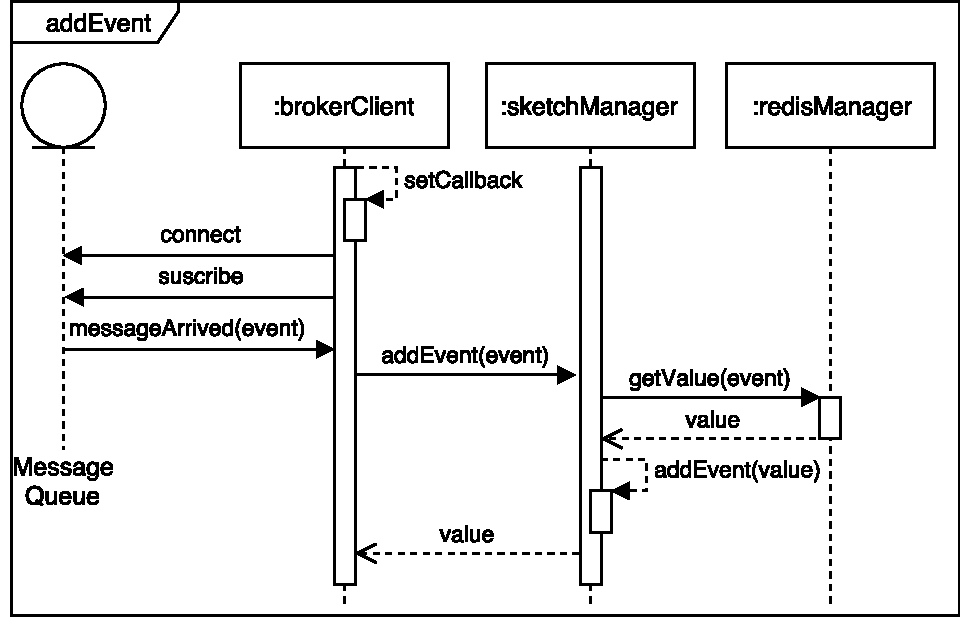
\includegraphics[width=0.45\textwidth]{./graph/SecDiag-resourceAddEventMosquitto.pdf}
	\caption{Diagrama de secuencia para nuevos eventos (tercer incremento)}
	\label{fig:SecDiagResourceAddEvent-Mosquitto}
\end{figure}

En la implementación anterior, los mensajes eran registrados directamente por un actor externo, mientras que ahora el sistema se suscribe a un canal particular de la cola de mensajes, escuchando nuevos eventos publicados en el mismo(es decir, usando comunicación indirecta). Mediante una función de \textit{callback} se especifica qué acción debe realizarse cada vez que el tópico notifica la llegada de un nuevo mensaje: este es agregado a un \textit{sketch} mediante  \textit{sketchManager} y procesado de igual forma que en la implementación del segundo incremento.
La figura \ref{fig:SecDiagResourceAddEvent-Mosquitto} muestra cómo el objeto \textit{brokerClient} implementa la lógica descrita anteriormente. Cuando es instanciado, el cliente debe conectarse a la cola de mensajes,  suscribirse a un tópico y configurar el \textit{callback}. También encapsula la lógica necesaria para manejar la pérdida o interrupción de la conexión al servicio.

\subsection{Reestructuración de código}
Otro aspecto importante a mejorar es la calidad del código del sistema. Esto no solo ayuda a mejorar ciertos aspectos funcionales como la eficiencia, sino que permite entender de manera sencilla los distintos módulos del sistema y la responsabilidad de cada uno de ellos. Así, el código es mucho más simple de interpretar, mantener y modificar.
El diagrama \ref{fig:system_components} muestra los diferentes componentes del sistema y la relación que existe entre ellos.

\begin{figure}[htbp]
	\centering
	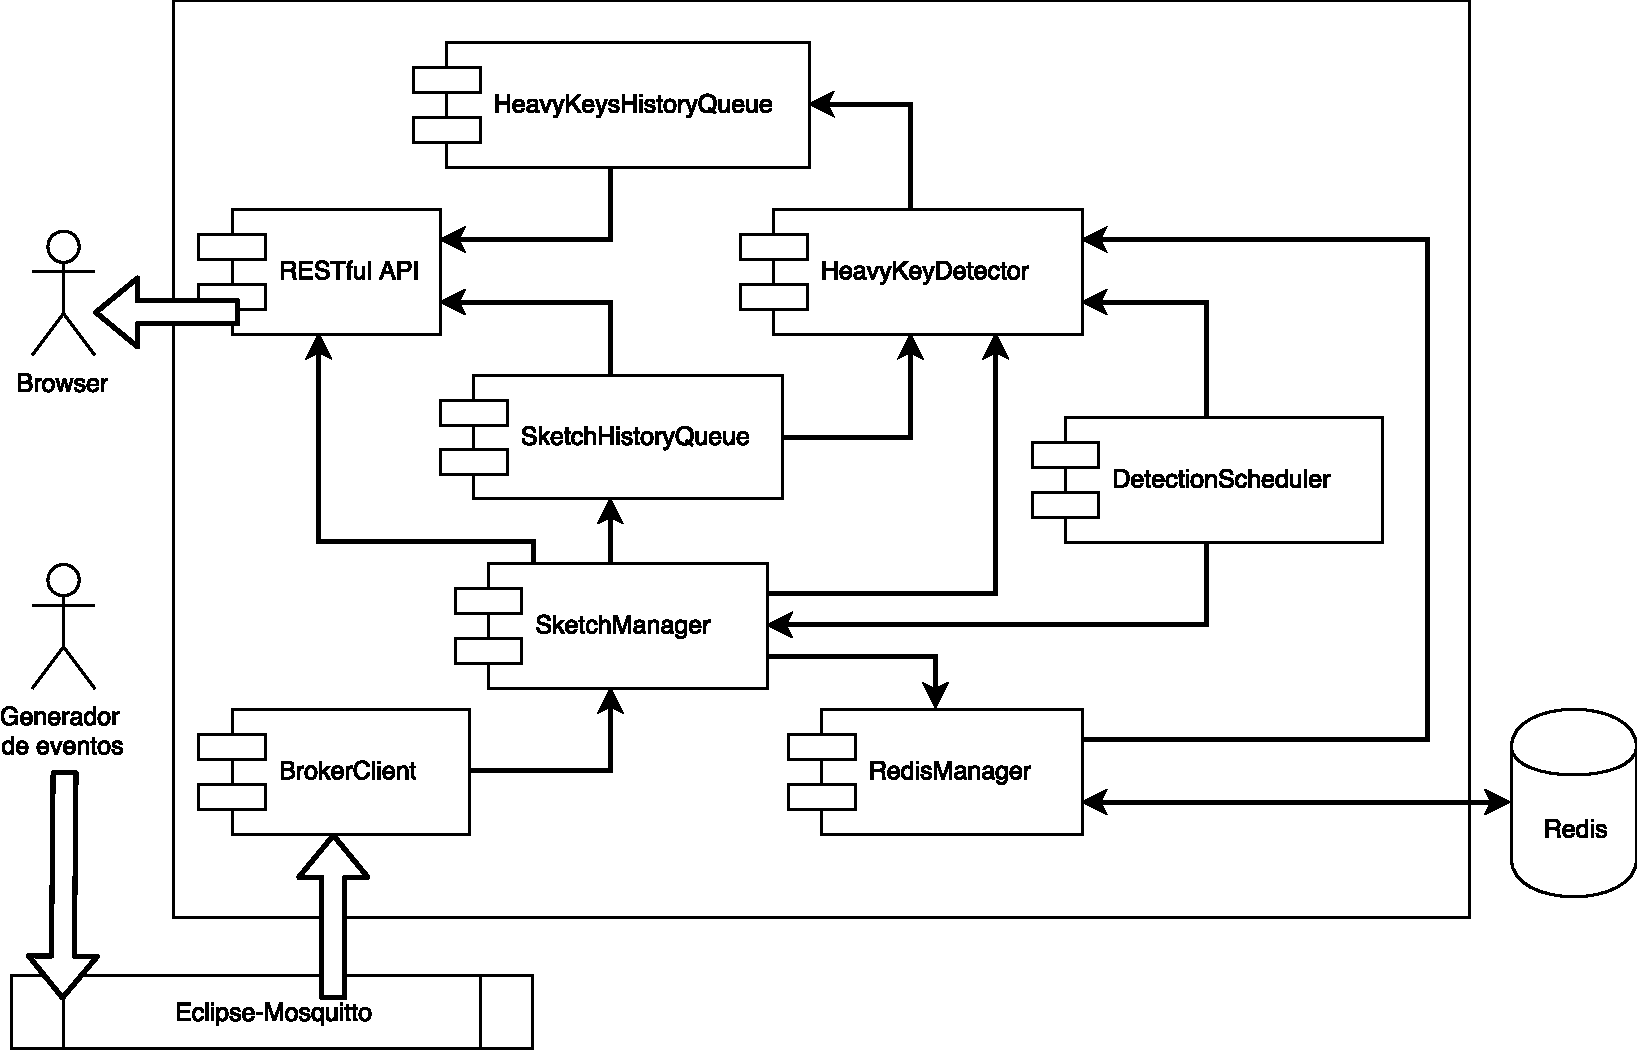
\includegraphics[width=0.9\textwidth]{./graph/system_components.pdf}
	\caption{Componentes del sistema y su interacción}
	\label{fig:system_components}
\end{figure}

Podemos describir la responsabilidad de cada módulo para comprender cómo funciona el servicio. El componente \textit{RedisManager} encapsula los métodos para conectar, consulta y almacenar datos en la base de datos clave-valor. Expone dos métodos para obtener los valores enteros asociados a un evento, y los eventos asociados a un conjunto de valores enteros. \textit{BrokerClient} envía los eventos que son publicados en un tópico a \textit{SketchManager}. Este último mantiene un objeto \textit{Sketch} activo en todo momento y actualiza su estado con cada nuevo evento procesado. Además, mediante \textit{RedisManager}, asigna un valor entero a cada evento registrado y persiste el par evento-valor en la base de datos.

Una vez transcurrida una ventana de tiempo o época, deben ejecutarse los métodos necesarios para detectar los eventos anómalos que están siendo procesados por el sistema. El componente \textit{DetectionScheduler} es el encargado de orquestar los diferentes pasos del algoritmo de detección implementado. Primero, indica al componente \textit{SketchManager} que una época a finalizado: este genera un nuevo objeto \textit{sketch} y almacena el objeto \textit{sketch} anteriormente activo en la cola \textit{SketchHistoryQueue}. Al mismo tiempo, el componente \textit{HeavyKeyDetector} es notificado del fin de la época: este toma los dos últimos \textit{sketch} disponibles en \textit{SketchHistoryQueue} y ejecuta los algoritmos de detección de eventos anómalos. Como la representación de los eventos en esta instancia son números enteros, deben recuperarse de la base de datos los eventos asociados a estos mediante \textit{RedisManager}. Finalmente, asocia los eventos detectados con la época de detección correspondiente, que es obtenida mediante \textit{SketchManager}.
Al finalizar la detección, \textit{HeavyKeyDetector} guarda los eventos detectados en la cola \textit{HeavyKeysHistoryQueue} para ser consultados convenientemente. Finalmente, se expone mediante una API REST los resultados de la detección junto con información del estado general del sistema.

\subsection{Exposición de los resultados de la detección}
A medida que los eventos son procesados el algoritmo de detección de eventos anómalos genera resultados en intervalos regulares de tiempo. Estos deben ser expuestos de manera conveniente para generar un visualización apropiada mediante una interfaz web. De esta forma, el sistema o \textit{backend} queda totalmente desacoplado de la visualización de la información o \textit{frontend}. Esto permite cambiar y mejorar los métodos de detección sin afectar su visualización, permitiendo de la misma manera cambiar la forma en que los datos son presentados sin necesidad de modificar el \textit{backend} en absoluto.
La información provista usando una REST API se enumera a continuación:
\begin{itemize}
	\item Estado general del sistema: valores de configuración, época actual de detección (número entero) y cantidad total de eventos procesados por el sistema.
	\item Información de cada época:  cantidad de elementos procesados y fecha de comienzo.
	\item Eventos detectados: fecha de finalización de cada época, cantidad de eventos anómalos detectados por época y los eventos detectados. Estos eventos son una lista de cadenas de caracteres o \textit{strings} para cáda época de detección.
\end{itemize}

Así, la interfaz web que será descrita en la siguiente sección, solo debe consumir estos datos y presentarlos de manera conveniente. Si lo pensamos desde el punto de vista de un modelo MVC (Model-View-Controller), el \textit{backend} resuelve el Model y el Controller, y el \textit{frontend} web resuelve la vista.

\section{Interfaz web}
Con las API correspondiente ofreciendo los resultados de la detección, solo resta implementar una vista de estos datos. Como la visualización de los datos pretende ser simple (emulando un \textit{dashboard}), se optó por implementar una aplicación web de página única, o SPA por \textit{Single-page Applicacion}. La ventaja principal de las SPA es que son dinámicas, lo cual evita refrescar la página para actualizar los datos mostrados, dando así una experiencia de aplicación de escritorio pero permitiendo ser usadas mediante un navegador, sin descargar programas adicionales.

Respecto a las tecnologías disponibles, existen dos estándares:
\begin{itemize}
	\item AngularJS: es un framework desarrollado y mantenido por Google Inc. Está escrito en JavaScript y hace uso del patrón de diseño MVC.
	\item ReactJS: es una librería para construir interfaces de usuario. Desarrollada y mantenida por Facebook, está pensada para diseñar vistas simples para cada estado de una aplicación. La librería es la encargada de actualizar y re-dibujar los componentes que sean necesarios cuando los datos cambian.
\end{itemize}

Si bien ambas tecnologías son ampliamente usadas y su desarrollo es sumamente activo, ReactJS parece ser la opción más conveniente dado que sus características se ajustan al problema que se intenta resolver, es decir, mostrar los datos provistos por el \textit{web-service} de manera dinámica, mientras que AngularJS ofrece un framework MVC completo que agregaría complejidad al desarollo.

En cuanto a cómo mostrar los datos, la primera aproximación consistió en el uso de una tabla con 5 columnas para fecha de detección, cantidad de \textit{Heavy Hitters}, los \textit{Heavy Hitters} detectados, cantidad de \textit{Heavy Changers} y los \textit{Heavy Changers} detectados. Sin embargo, cómo la cantidad de eventos detectados por fila es variable, hubiese sido necesario mostrar más de una dato por celda, por lo que la utilización de una tabla parecería no ser la adecuada (se asume que cada celda es atómica, es decir, debe mostrar un único dato).

Otra alternativa mas conveniente dada la naturaleza temporal de los datos, y la cantidad de ocurrencia de eventos, es utilizar un histograma con desplazamiento. Con cada desplazamiento, los datos para la nueva época son agregados. Así, puede observarse cuando ocurren ciertos eventos, y compararlos a simple vista con otros intervalos de tiempo pasados y futuros. En la imagen \ref{fig:ui} puede observase una primera implementación de la interfaz web.

\begin{figure}[htbp]
	\centering
	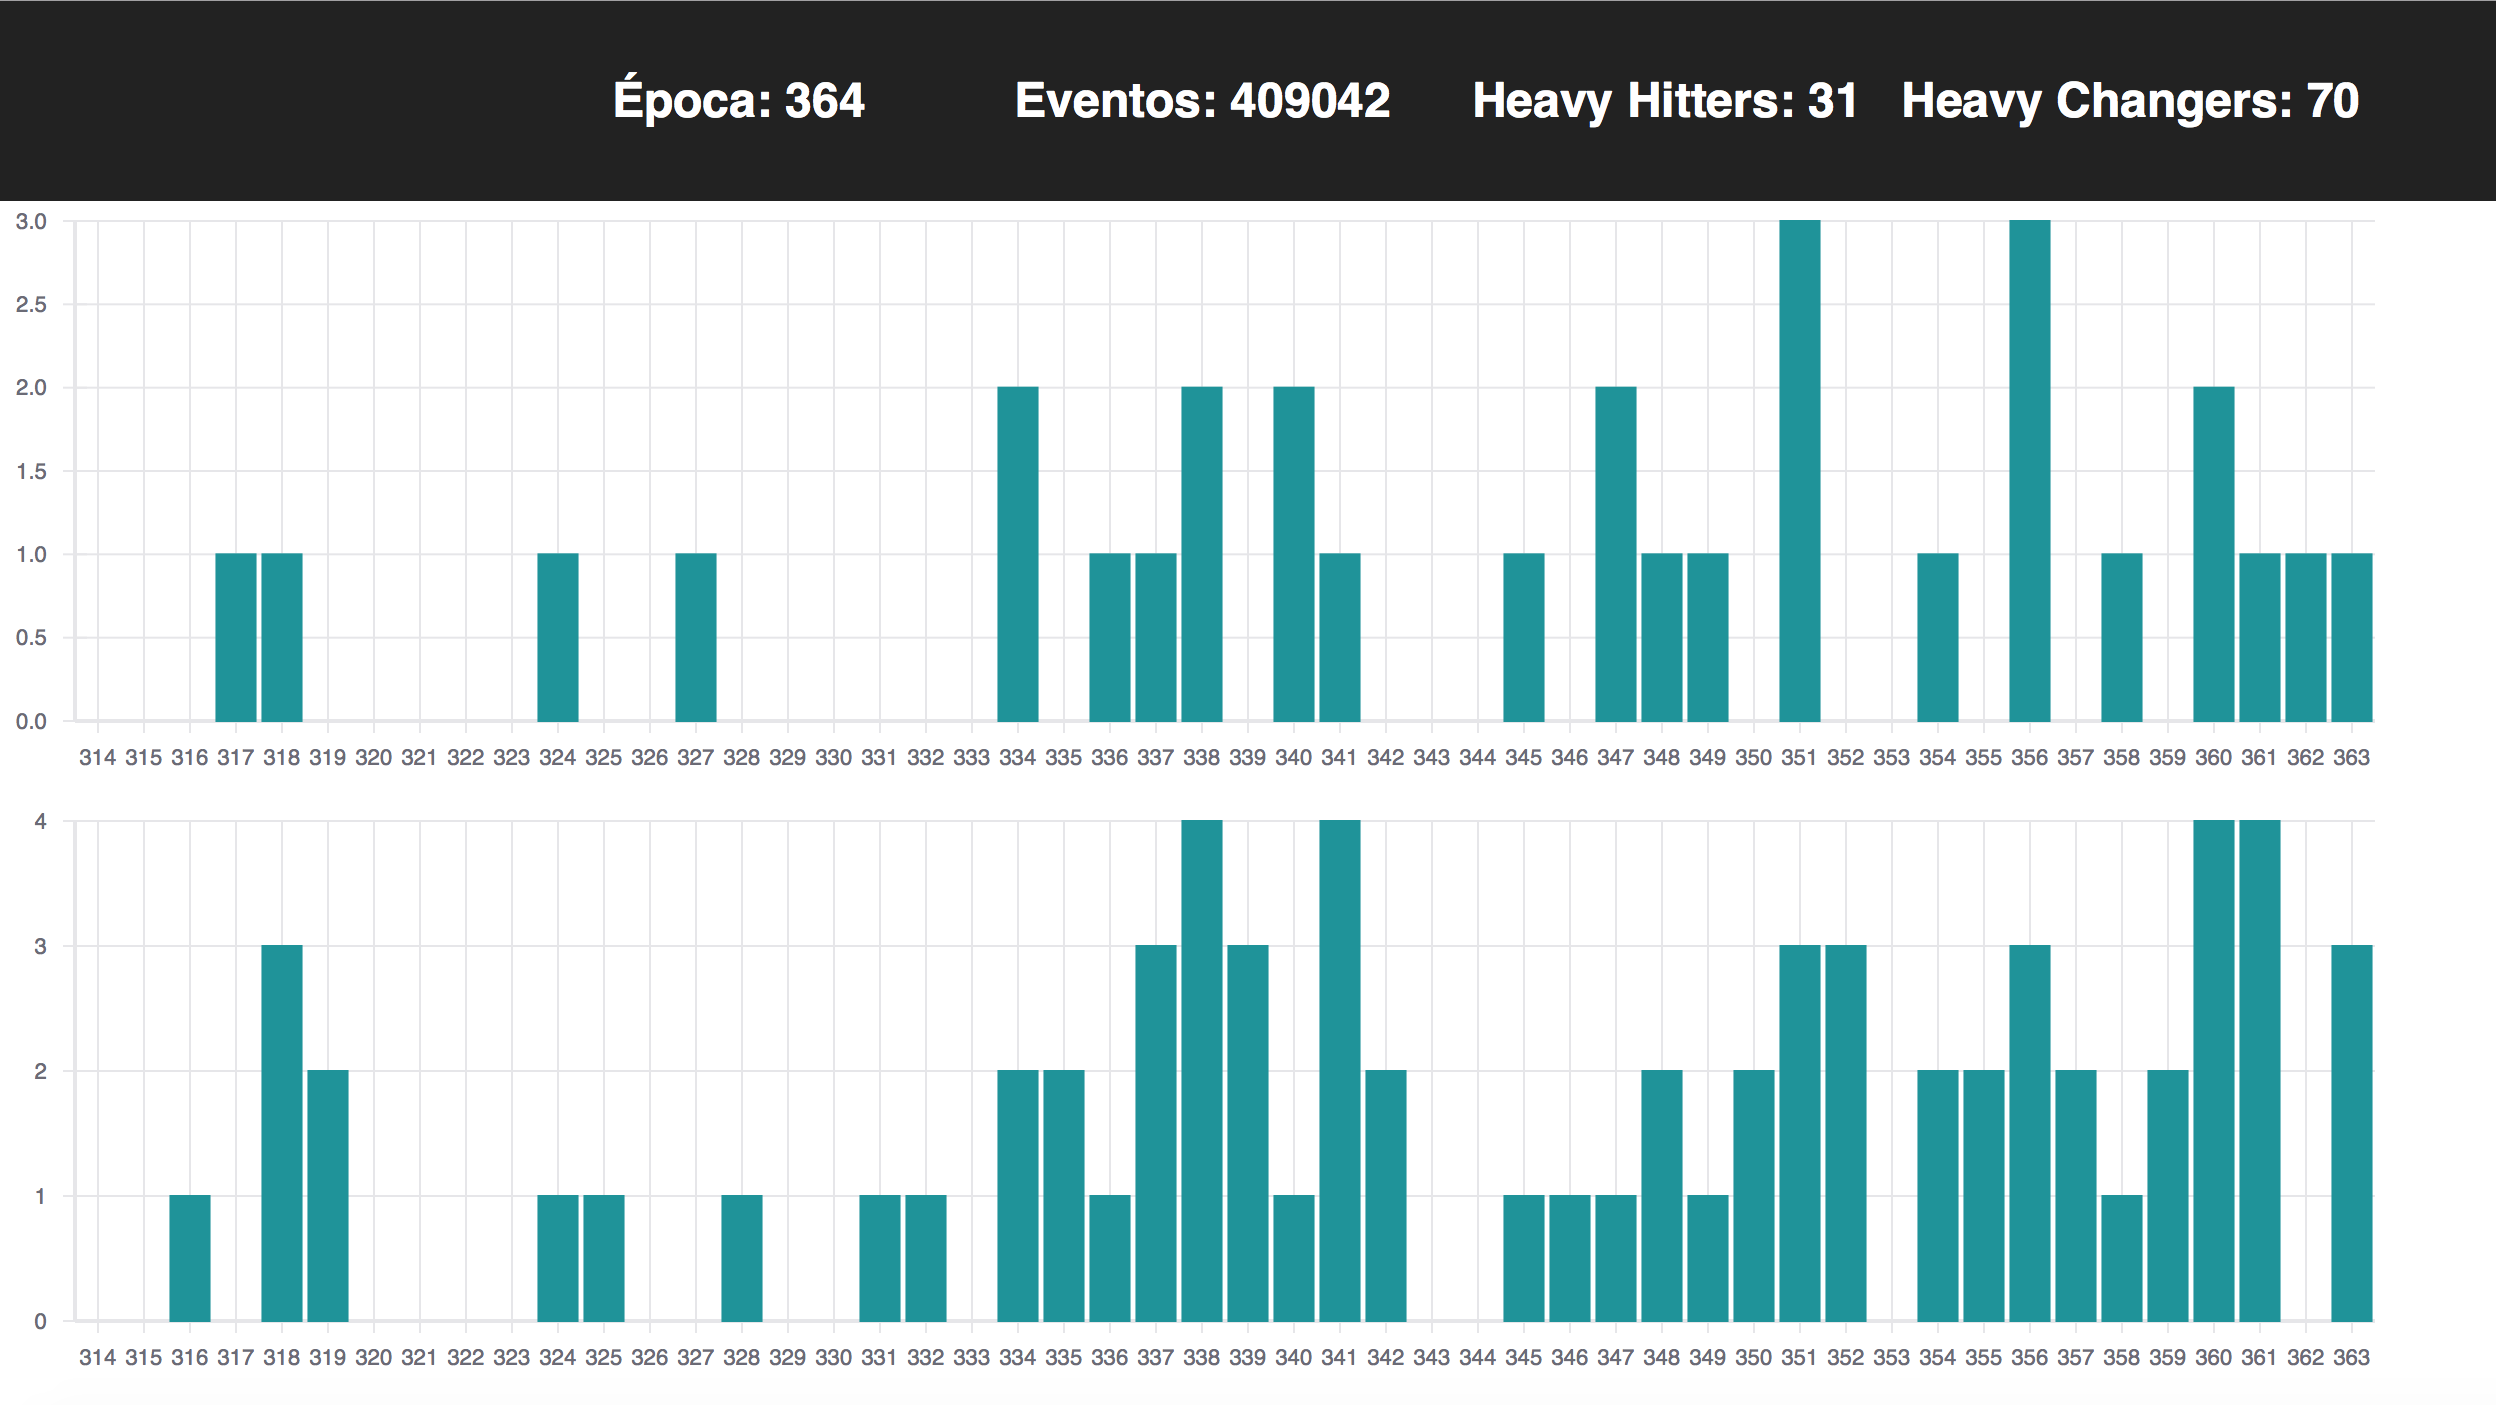
\includegraphics[width=0.9\textwidth]{./graph/ui.png}
	\caption{Interfaz web del sistema}
	\label{fig:ui}
\end{figure}

En el panel superior pueden observarse los datos generales del sistema: época que está siendo computada, cantidad de eventos totales procesados y la cantidad de \textit{heavy keys} encontradas hasta el momento. El primer histograma muestra cuantos \textit{heavy hitters} ocurrieron en cada época y el segundo muestra cuando \textit{heavy changers} fueron identificados. Queda pendiente elegir definir es la mejor forma de visualizar las etiquetas de los eventos detectados y mejorar la descripción de los datos en la interfaz.

\section{Conclusiones}
En este incremento se realizaron una cantidad considerable de modificaciones al código. Como es usual en los desarrollos ágiles, primero se parte de una prueba de concepto para mostrar el valor que puede entregar un sistema o algoritmo, y luego se trabaja en mejorar aspectos técnicos para hacer de la misma una idea productizable.
En particular, podemos observar que las mejoraras en \textit{performance} son más que satisfactorias. Si bien para el presente informe sólo se usaron datos sintéticos y de tráfico de red, el mismo método puede aplicarse en diferentes aplicaciones: e-commerce (determinar en tiempo real artículo es el mas buscado) o análisis de texto en tiempo real (cuales son las palabras más usadas en todo momento), por nombrar algunos.
Por otro lado, la integración de una \textit{message queue} en el sistema fue fundamental, no solo para incrementar las prestaciones del servicio, sino para permitir escalabilidad: ante grandes volúmenes de eventos enviados al servicio, la carga es soportada por la \textit{message queue}, lo cual evita agregar esta lógica al servicio desarrollado.
Finalmente, la interfaz web muestra, en una sola vista, toda la actividad detectada por el sistema y permite a usuario observar cual es el estado general de los eventos que está analizando, sin necesidad de interactuar con la interfaz.
\newpage
\nocite{*}
\printbibliography

\end{document}

